% !TeX root = ./jvk-blatt1.tex

\excercise{Task und UI}
\label{ex3}

\begin{enumerate}
    \item Nun wollen wir wie in Aufgabe 1 ein Spiel starten. Dazu ersetzen wir den \lstinline{ new demoTask} und \lstinline{new demoTaskVerifier} in der Main Klasse, durch 
        den \lstinline{Sheet1Task3} wie hier gezeigt:

    \begin{lstlisting}
Game demoGame = new Game("Hello World", new Sheet1Task3());
    \end{lstlisting}

    Du startest das Spiel in der Variable \lstinline{demoGame} indem du die Operation \lstinline{run()} darauf aufrufst.

    \begin{lstlisting}
demoGame.run();
    \end{lstlisting}

    Starte das Programm in Eclipse, mit dem kleinen Play-Button oben in der Werkzeugleiste und schau dich ein wenig im Fenster, das dann aufgeht um.

    \vspace{5mm}

    \item In der vorherigen Teilaufgabe hattest du bereits ''Hello World'' und ein Task Objekt an Game übergeben.
        Nun wollen wir noch ein TaskVerifier Objekt übergeben.\\
        Orientiere dich dazu unten am Bild. Starte nachdem du fertig bist das Spielfenster neu. \\

        Was verändert sich im Spielfenster?
        Finde den \q{Task Status} Tab und drücke den Refresh Button.

    \begin{lstlisting}
Game demoGame = new Game("Hello World", new Sheet1Task3(), new Sheet1Task3Verifier());
    \end{lstlisting}

\end{enumerate}


\begin{Infobox}[Der Refresh Button]
    Wenn du überprüfen willst, ob du deine Aufgabe erledigt hast, musst du den \fbox{Task Status} Tab unter dem Spielfeld öffnen und dann auf \fbox{Refresh} klicken.\\

    Wichtig: Der Task Status aktualisiert sich nicht automatisch. Du musst also immer selber aktualisieren.
\end{Infobox}


\begin{enumerate}\setcounter{enumi}{2}

    \item Finde sowohl im Spiel als auch in Eclipse die Konsole. Dies ist ein Feld in dem Text ausgegeben wird:
    \begin{center}
        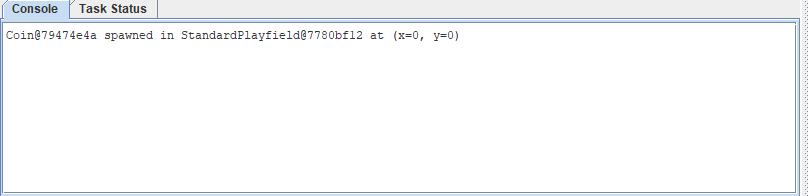
\includegraphics[width=\linewidth]{./figures/console.PNG}
    \end{center}

    In der Konsole siehst du, dass eine Münze (\texttt{Coin}) gespawnt (erzeugt) wurde.
    Finde die Koordinaten des Feldes, auf welchem die Münze gespawnt wurde.

    \item Nun suche nach der Stelle im Code in der Klasse \lstinline{Sheet1Task3}, in dem die erste Münze erzeugt wird.\\
    Hinweis: \lstinline{Sheet1Task3} findest du im \lstinline{project/src/main/java/de/unistuttgart/informaitk/fuis/jvk/tasks}-Ordner des Projektes.

    \item Nun wollen wir endlich mal selber Münzen auf das Spielfeld platzieren.
        Hierfür bearbeitest du die Klasse \lstinline{Sheet1Task3}.\\
        Platziere mindestens 5 Münzen auf beliebigen Feldern.

        Benutze den \q{Task Status} um herauszufinden, ob du die Aufgabe erfolgreich gelöst hast.

        Wie ist der Zusammenhang zwischen Position der Münze und die Koordinaten im Koordinatensystem?

        \textbf{Tipp:} Wenn du nicht genau weißt, wie man eine Münze erzeugt, schaue dir den Code, welchen du in Teilaufgabe d) gefunden hast, nochmal an.
    \item Du kannst auch im Fenster selbst Münzen und Wände platzieren, dies geht rechts oben mit dem + und - Button. Versuche die Aufgabe e) nun nochmal zu lösen ohne im Code Münzen zu platzieren.
\end{enumerate}
